\subsection{The acceptance deadline and observation periods}
\label{sec:event-history}

A team needs two dates to relate retained output to labour. The first is the task's output assessment date. For a task accepted by the deadline, a reviewer checks its requirement at age $T_i+\Delta$. The second is the end of labour observation. Every task contributes attributable hours through age $\tau+\Delta$, including tasks that miss the deadline.

Figure~\ref{fig:task-clocks} shows a task accepted on day three of a fourteen-day acceptance window. Fourteen days after acceptance, the reviewer checks which parts of the requirement still hold. The assessment therefore falls on day seventeen. Repair on day twenty still contributes to labour because the common labour period ends on day twenty-eight. Adding the task's start time $s_i$ to each age places its work on the same calendar as other tasks that share the team.

% Illustrative accepted task: T_i=3 days, tau=14 days, Delta=14 days.
% Hence output assessment is at day 17, and the labour total includes work through day 28.
% Text alternative: acceptance by day fourteen qualifies the task for output;
% its day-three acceptance starts fourteen-day follow-up. Labour is counted
% from day zero through day twenty-eight, including work after the output check.
\begin{figure}[htp]
\centering
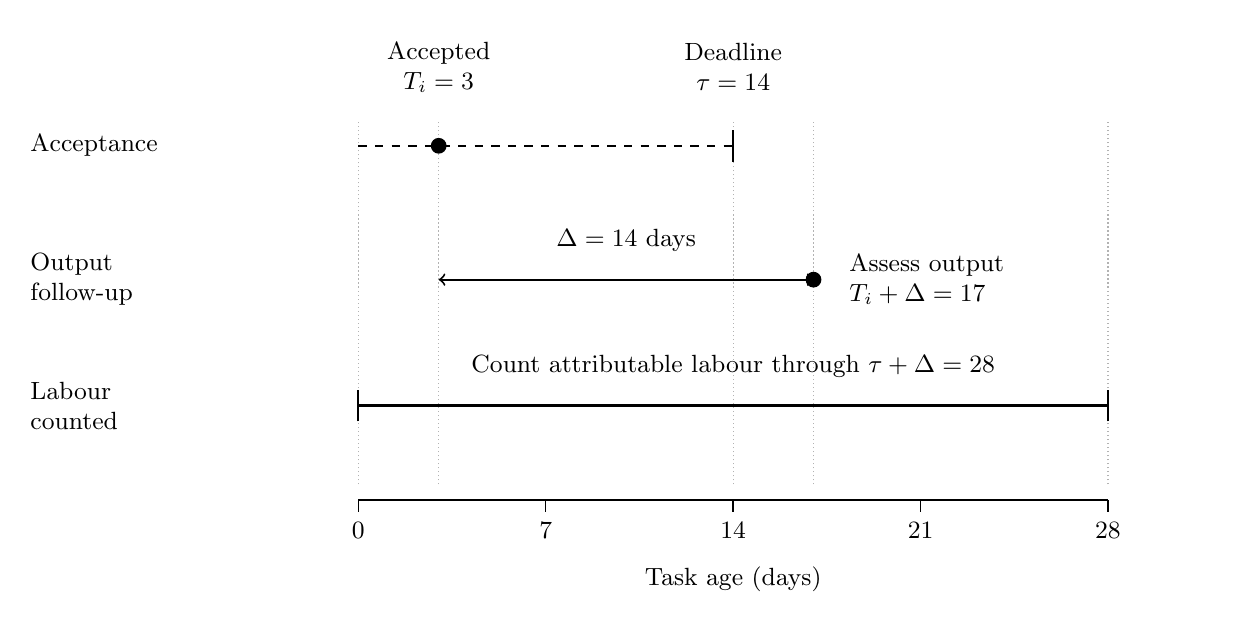
\begin{tikzpicture}[x=1mm,y=1mm,font=\fontsize{9}{11}\selectfont,
  every node/.style={inner sep=1pt,outer sep=0pt}]
  \path[use as bounding box] (0,-8) rectangle (152.4,65);
  \node[anchor=west] at (0,50) {Acceptance};
  \node[anchor=west,align=left] at (0,33) {Output\\follow-up};
  \node[anchor=west,align=left] at (0,17) {Labour\\counted};
  \foreach \day in {0,3,14,17,28} {
    \draw[black!30,densely dotted,line width=0.45pt]
      ({42+3.4*\day},7) -- ({42+3.4*\day},53);
  }
  \draw[dashed,line width=0.7pt] (42,50) -- (89.6,50);
  \fill (52.2,50) circle (1mm);
  \draw[line width=0.7pt] (89.6,48) -- (89.6,52);
  \node[align=center] at (52.2,60) {Accepted\\$T_i=3$};
  \node[align=center] at (89.6,60) {Deadline\\$\tau=14$};
  \draw[<->,line width=0.7pt] (52.2,33) -- (99.8,33);
  \node at (76,38) {$\Delta=14$ days};
  \fill (99.8,33) circle (1mm);
  \node[anchor=west,align=left] at (104,33) {Assess output\\$T_i+\Delta=17$};
  \draw[line width=1pt] (42,17) -- (137.2,17);
  \foreach \xx in {42,137.2} {
    \draw[line width=0.7pt] (\xx,15) -- (\xx,19);
  }
  \node at (89.6,22) {Count attributable labour through $\tau+\Delta=28$};
  \draw[line width=0.5pt] (42,5) -- (137.2,5);
  \foreach \day in {0,7,14,21,28} {
    \draw[line width=0.5pt] ({42+3.4*\day},5) -- ({42+3.4*\day},3.5);
    \node[anchor=north] at ({42+3.4*\day},2.5) {\day};
  }
  \node at (89.6,-5) {Task age (days)};
\end{tikzpicture}
\caption{\textbf{An early acceptance brings the output check forward.}
With $\tau=14$ and $\Delta=14$ days, acceptance on day three puts the output check on day seventeen. The solid line covers the labour observation period through day twenty-eight. Work on the task at any time during that period contributes person-hours, including repairs after the output check. Adding $s_i$ to an age on the horizontal axis gives the corresponding calendar time.}
\label{fig:task-clocks}
\end{figure}

